\chapter{Funktionsweise von Spark}
\label{chapter:funktionsweise von Spark}



Wie in Abbildung 3 dargestellt, werden die Daten bei einer Verarbeitung durch Spark zunächst aus dem HDFS geladen, in Resilient Distributed Datasets (RDD) verpackt, und dann im Hauptspeicher für Verarbeitung- oder Analysefunktionen zur Verfügung gestellt. Abfragen werden direkt entweder via Scala REPL oder SQL-artige Abfragen zur Laufzeit, über Batch-Jobs oder via Spark Streaming/Storm an die im RAM befindlichen RDDs geleitet.

\begin{figure}[htb!]
\centering
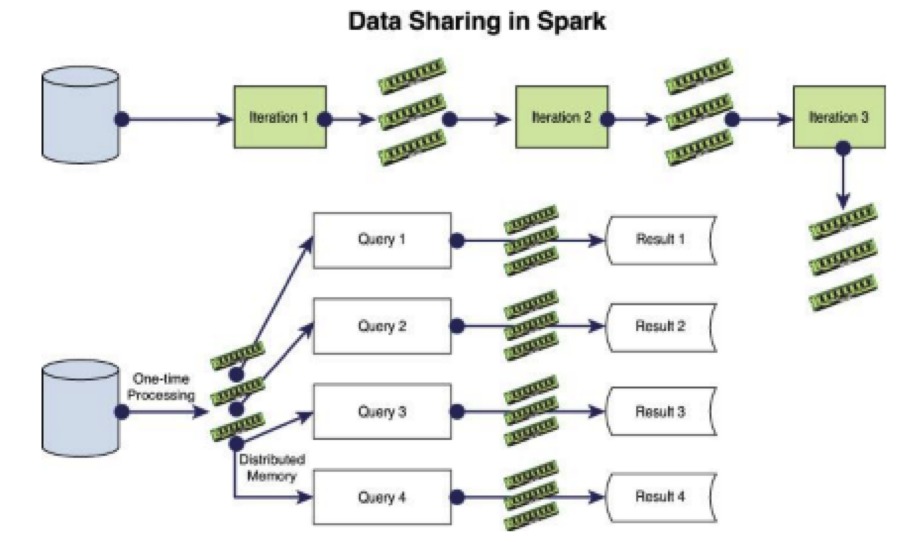
\includegraphics[width=1.0\textwidth]{bilder/3_spark.png}
\caption{Schematische Darstellung der Funktionsweise von Spark [VA14]}
\label{fig:sparkfunkt}
\end{figure}
  
\section{Das Konzept der RDD}
\label{section:rdd}



Bei den Resilient Distributed Datasets (RDD) in Spark handelt es sich um verteilte Objekt-Collections, die im Allgemeinen im Speicher der Cluster-Knoten gecached  und zwischen den Knoten bewegt werden. Sie können durch verschiedenste parallele Operatoren manipuliert und im Fehlerfall automatisch neu aufgebaut werden. Deshalb merken sich die RDDs die Transformationen, die zu ihrem Aufbau geführt haben und können so verlorene Daten schnell rekonstruieren. Da es sich bei RDDs prinzipiell um Scala-Collections handelt, können diese auch direkt in Scala-Code eingebunden und verarbeitet werden, oder interaktiv über die Scala-Konsole REPL genutzt werden. RDDs können nur durch 




grobgranulare, deterministische Transformationen, wie beispielsweise map, filter, join, etc. erstellt werden. 

RDDs können prinzipiell auf drei Arten gespeichert werden [SP14]:
\begin{itemize}
		\item Als deserialisiertes Java-Objekt im Speicher der JVM – dieses Variante bietet die beste Performance, da die Objekte sich direkt im JVM-Heap befinden
		\item Als serialisiertes Java-Objekt direkt im Speicher – dieses Verfahren ist speicher-effizienter, aber schlechter in der Zugriffsgeschwindigkeit
		\item Im Dateisystem – diese Variante ist erwartungsgemäß die langsamste, jedoch nötig, wenn die RDDs zu groß für die Haltung im RAM sind. 		
\end{itemize}	





\section{Spark im Cluster}
\label{section:spark im cluster}


Spark-Anwendungen laufen als unabhängiges Set von Prozessen auf Cluster-Infrastrukturen. Das Hauptprogramm (Driver-Program) enthält das SparkContext-Objekt, das die einzelnen Prozesse koordiniert. Auf Clustersystemen hält der SparkContext die Verbindung zum jeweiligen Cluster-Manager (Mesos, Yarn), im Standalone-Betrieb instanziert der Context selbst einen Dummy-Manager und allokiert in beiden Fällen die für die Anwendung nötigen Hardware-Ressourcen.    

\begin{figure}[htb!]
\centering
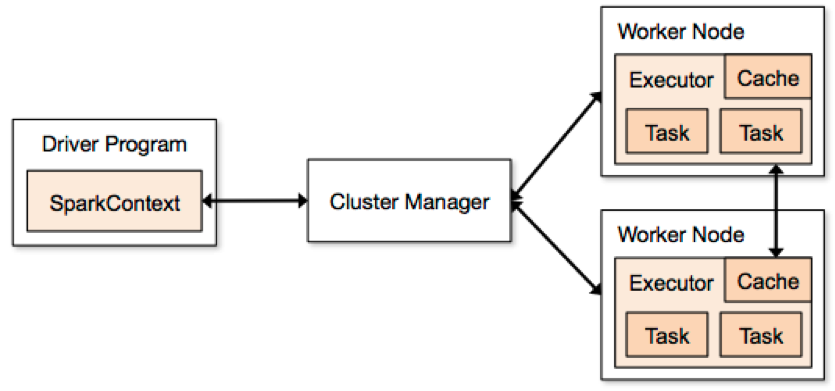
\includegraphics[width=1.0\textwidth]{bilder/3_2_cluster.png}
\caption{Clusteraufbau mit Spark [SP14]}
\label{fig:sparkcluster}
\end{figure} 






Wenn eine Verbindung aufgebaut ist, installiert Spark sogenannte Executors auf den Knoten des Clusters. Der Applikationscode wird nun als JAR direkt an die Executors geschickt und dieser anschließend durch entsprechende Tasks ausgeführt. 
































